\documentclass[10pt]{article}

\usepackage[utf8x]{inputenc}
\usepackage[english,italian]{babel}
\usepackage{graphicx} 
\usepackage{booktabs}
\usepackage{caption}
\usepackage{textgreek}
\usepackage{tabularx}
\usepackage{amsmath,amssymb,stackengine}
\usepackage{authblk}
\usepackage{xcolor}


\usepackage{geometry} % to change the page dimensions
\geometry{a4paper} % or letterpaper (US) or a5paper or....
% \geometry{margin=2in} % for example, change the margins to 2 inches all round
% \geometry{landscape} % set up the page for landscape
%   read geometry.pdf for detailed page layout information

\usepackage{graphicx} % support the \includegraphics command and options

% \usepackage[parfill]{parskip} % Activate to begin paragraphs with an empty line rather than an indent

%%% PACKAGES
\usepackage{booktabs} % for much better looking tables
\usepackage{array} % for better arrays (eg matrices) in maths
\usepackage{paralist} % very flexible & customisable lists (eg. enumerate/itemize, etc.)
\usepackage{verbatim} % adds environment for commenting out blocks of text & for better verbatim
\usepackage{subfig} % make it possible to include more than one captioned figure/table in a single float
% These packages are all incorporated in the memoir class to one degree or another...

%%% HEADERS & FOOTERS
\usepackage{fancyhdr} % This should be set AFTER setting up the page geometry
\pagestyle{fancy} % options: empty , plain , fancy
\renewcommand{\headrulewidth}{0pt} % customise the layout...
\lhead{}\chead{}\rhead{}
\lfoot{}\cfoot{\thepage}\rfoot{}

\usepackage{sectsty}
\allsectionsfont{\sffamily\mdseries\upshape} 

\usepackage[nottoc,notlof,notlot]{tocbibind}
\usepackage[titles,subfigure]{tocloft} 

\renewcommand{\cftsecfont}{\rmfamily\mdseries\upshape}
\renewcommand{\cftsecpagefont}{\rmfamily\mdseries\upshape} 
\newcommand*{\hham}{\mathcal{H}}
\newcommand*{\xx}{\vec{x}}
\newcommand*{\kk}{\vec{k}}
\newcommand*{\qq}{\vec{q}}
\newcommand*{\p}{\varphi}
\newcommand*{\zpart}{\mathcal{Z}}
\newcommand*{\w}{\Bigl}
\newcommand*{\lapint}{\int_{a-i\infty}^{a+i\infty}\frac{dz}{2\pi i}}

\definecolor{carmine}{rgb}{0.59, 0.0, 0.09}


\selectlanguage{english}

\title{{\bf Notes on ecosystems stability}}

\author{Onofrio Mazzarisi}

%\affil{{\it Max Planck Institute for Mathematics in the Sciences, Leipzig, Germany}}

\begin{document}

\selectlanguage{english}

%\begin{abstract}
%\end{abstract}

\maketitle

\section{$\alpha\beta\gamma$-model}

Consider a competitive community of $S$ species
defined by the following dynamics for the population densities
\begin{equation}
    \frac{dn_i}{dt}=n_i^{\alpha}-n_i^{\beta}\sum_{j}A_{ij}n_j^{\gamma} \, ,
\end{equation}
where the sum runs from $j=1$ to $j=S$ and the off-diagonal elements
of $A$ are extracted from a distribution
with mean $\mu>0$ and standard deviation $\sigma$ while $A_{ii}=1/K$, $\forall i$,
$K$ being the (uniform) carrying capacity.
(To be more precise $K^{1/(\beta+\gamma-\alpha)}$ is the carrying capacity).
If the equilibrium is feasible it formally reads
\begin{equation}
    (n_i^*)^{\alpha-\beta} = \sum_{j}A_{ij}(n_j^*)^{\gamma} \, .
\end{equation}
The element of the jacobian for $j\neq i$ read
\begin{equation}
    J_{ij} = -\gamma n_i^{\beta}A_{ij}n_j^{\gamma} \, ,
\end{equation}
while the diagonal components read
\begin{equation}
    J_{ii} = \alpha n_i^{\alpha-1}-\beta n_i^{\beta-1}\sum_{j\neq i}A_{ij}n_j^{\gamma}
    - (\beta+\gamma)A_{ii}n_i^{\beta+\gamma} \, .
\end{equation}

\subsection{Uniform case}
In the case of uniform interactions ($\sigma=0$)
the species population are all equal and the equilibrium reads
\begin{equation}
    n^*=\left[\mu(S-1)+\frac{1}{K}\right]^{1/(\alpha-\beta-\gamma)} \, .
\end{equation}
The jacobian evaluated at equilibrium is
\begin{equation}
    J_{ij}\Big{|}_{n=n^*} = -\gamma \mu (n^*)^{\beta+\gamma-1} \, ,
\end{equation}
\begin{equation}
    J_{ii}\Big{|}_{n=n^*} = \alpha (n^*)^{\alpha-1}-\beta (n^*)^{\beta+\gamma-1}\mu(S-1)
                            -\frac{(\beta+\gamma)}{K}(n^*)^{\beta+\gamma-1}\, .
\end{equation}

The maximum eigenvalue $\lambda_{\textrm{max}}$ is $S-1$ degenerate and reads formally
\begin{equation}
    \lambda_{\textrm{max}} = J_{ii}\Big{|}_{n=n^*} - J_{ij}\Big{|}_{n=n^*} \, .
\end{equation}
The stability condition
\begin{equation}
    \lambda_{\textrm{max}} = \alpha (n^*)^{\alpha-1}-(n^*)^{\beta+\gamma-1}\left[\beta \mu(S-1)
    +\frac{(\beta+\gamma)}{K}-\gamma\mu\right]<0 \, ,
\end{equation}
can be written as
\begin{equation}
    \alpha (n^*)^{\alpha-\beta-\gamma}-\left[\beta \mu(S-1)
    +\frac{(\beta+\gamma)}{K}-\gamma\mu\right]<0 \, ,
\end{equation}
which, using the expression for $n^*$ and after some manipulations reads
\begin{equation}
    (S-1)(\beta-\alpha) > \frac{K\mu\gamma+\alpha-\beta-\gamma}{K\mu} \, .
\end{equation}
We have then three possibilities:
\begin{align}
    S &> 1 + \frac{K\mu\gamma+\alpha-\beta-\gamma}{K\mu(\beta-\alpha)} 
    &\textrm{if} \quad \beta/\alpha>1 \, , \\
    S &< 1 + \frac{K\mu\gamma+\alpha-\beta-\gamma}{K\mu(\beta-\alpha)} 
    &\textrm{if} \quad \beta/\alpha<1 \, , \\
    \mu &< \frac{1}{K} &\textrm{if} \quad \beta/\alpha=1 \, .
\end{align}
A series of comments is in order. 
\begin{itemize}
    \item Depending on $\beta/\alpha$ we have \textit{two
    regimes}: one in which increasing $S$ enhances stability ($\beta/\alpha>1$) and 
    one in which it hinders stability ($\beta/\alpha<1$).
    Notably this is independent from $\gamma$, indicating that only the interplay between
    the density dependence of the contribution of a species to the interactions and
    the density dependence of its production term that is (qualitatively) relevant; 
    and not the form of the contribution of the competitors to the interactions.
    \item The critical case ($\beta/\alpha=1$) not only recovers the usual GLV result
    but \textit{generalize it}, indeed it does not depend on $\gamma$ which cancels out.
    \item For $K\to\infty$ and $\beta=1$ we recover the result
    \begin{equation}
        S=1+\frac{1}{1-\alpha} \, ,
    \end{equation}
    once again \textit{independently} on $\gamma$.
\end{itemize}

Being the specification of $\gamma$ 
mostly irrelevant, for symmetry reason it is probably sensible to consider 
models with $\gamma=\beta$,
leaving the potential asymmetry of the competitive interaction between two species
to the coefficient $A_{ij}$.

\subsection{Non-uniform case}

\section{On sublinear production}
Observations point towards a sublinear production scaling
with respect to the population biomass density. 
This observations may refer to
dynamical production or to the equilibrium production observed
across a biomass gradient.

Here we discuss how dynamical sublinear production does not generally leads to 
sublinear production across a biomass gradient.
Nonetheless, although not sufficient, it might be necessary for (or at least
functional to) sublinear scaling across a biomass gradient.

\subsection{Single population}
Let us focus on a single population example to calrify the ideas.
Consider a production function of the form
\begin{equation}
    P(n) = r n^\alpha \, ,
\label{eq: production}
\end{equation}
where $n$ is the biomass density of the population, $\alpha\leq1$
specify the intensity of sublinear dynamical scaling (linear when $\alpha=1$) 
and $r$ is the parameter that allows to move across a biomass gradient.
Consider then a loss term of the form
\begin{equation}
    L(n) = s n^\beta \, .
\end{equation} 
The evolution equaiton for the population is 
\begin{equation}
    \frac{dn}{dt} = P(n) - L(n) = r n^\alpha - s n^\beta \, ,
    \label{eq: single}
\end{equation} 
which reduces to logistic growth for $\alpha=1$ and $\beta=2$.
The equilibrium is given by
\begin{equation}
    n^* = \left(\frac{r}{s}\right)^{1/(\beta-\alpha)} \, ,
\label{eq: equilibrium single}
\end{equation}
and the stability condition is given by
\begin{equation}
    \frac{d\left[P(n)-L(n)\right]}{dn}\bigg|_{n=n^*} < 0 \, ,
\end{equation}
which leads, after some calculations, to the condition
\begin{equation}
    \alpha<\beta \, ,
\end{equation}
independent from $r$ and $s$.

It possible to appreciate from Eq.~(\ref{eq: equilibrium single})
that $\alpha>\beta$, apart from making the equilibrium unstable, implies that
the stationary population \textit{decreases} for increasing $r$,
which is biologically unreasonable.

The equilibrium production scales, at varying growth rate $r$,
as $P(n^*)=s(n^*)^\beta$ as can be noted by Eq.~(\ref{eq: equilibrium single})
for $r$ and then substituting it in the defining Eq.~(\ref{eq: production})
or simply by considering the dynamical equation at stationarity.
Notice that, if $s$ is varied instead, the exponent
of dynamical and across-biomass-gradient production coincide.
Figure~\ref{fig. example} shows an example with specific parameters.

\begin{figure}[h!]
    \centering
    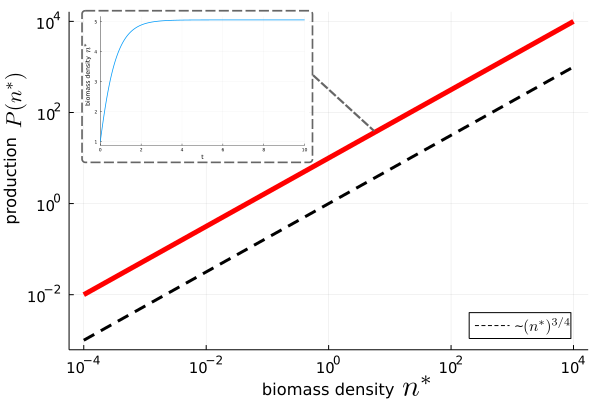
\includegraphics[width=.8\textwidth]{fig/single-pop.pdf}
    \caption{Production versus biomass density in single population descirbed in
    Eq.~(\ref{eq: single}) for $r\in[1,100]$,
    $s=10$, $\alpha=1/2$ and $\beta=3/4$. In the inset the equilibration process
    for $r=10$.}
    \label{fig. example}
\end{figure}

In summary, for an environmental change that amount to a change in $r$, 
the production across a biomass gradient 
scales as $(n^*)^\beta$. In order for
the stationary solution to be stable an exponent $\alpha<\beta$
for the dynamical produciton is needed.
Therefore, in order to have sublinear $P(n^*)$ across a biomass gradient,
we need $\alpha<\beta<1$.
If the increment of the equilibrium biomass density is due to decreasing $s$,
equilibrium and dynamical production scale in the same way and in order to
have sublinear $P(n^*)$ we need $\alpha<1$ with $\alpha<\beta$ for stability
but no constraint on $\beta$. Either way we need $\alpha<1$.

\subsection{Competitive community}

Consider the $\alpha\beta\gamma$-model

\section{$(\sigma\sqrt{S},\mu S)$ plane}


\section{General production with GLV interactions}
Consider the system of $S$ species
\begin{equation}
    \frac{dn_i}{dt} = P(n_i) - n_i\sum_{j\neq i}A_{ij}n_j \, ,
\end{equation}
where the summation runs over all the species and we leave the production function generic
and $A$ is a matrix with zero diagonal and off-diagonal elements gaussianly
ditrubuted with mean $\mu$ and standard deviation $\sigma$.
The community matrix reads in this case
\begin{equation}
    C = -D(n^*)A - D(P(n^*)/n^*-P'(n^*)) \, ,
\end{equation}
where the notation $D(x)$ stands for a diagonal matrix filled 
with the components of the vector
$x$ and $P(n^*)=(P(n_1^*), ..., P(n_S^*))$ and $P'(n^*)=(dP(n_1^*)/dn_1^*, ..., dP(n_S^*)/dn_S^*)$.

We have instability when
\begin{equation}
    \sum_i \frac{1}{|\mu -P(n_i^*)/(n_i^*)^2+P'(n_i^*)/n_i^*|^2}\geq 1/\sigma^2 \, .
\end{equation}

\newpage

\bibliography{Bib/library.bib}

\bibliographystyle{unsrt}

\end{document}